\documentclass[a0,portrait]{a0poster}
\usepackage{multicol} % This is so we can have multiple columns of text side-by-side
\columnsep=100pt % This is the amount of white space between the columns in the poster
\columnseprule=3pt % This is the thickness of the black line between the columns in the poster

\usepackage[svgnames]{xcolor} % Specify colors by their 'svgnames', for a full list of all colors available see here: http://www.latextemplates.com/svgnames-colors

\usepackage{times} % Use the times font
%\usepackage{palatino} % Uncomment to use the Palatino font

\usepackage{graphicx} % Required for including images
\graphicspath{{figures/}} % Location of the graphics files
\usepackage{booktabs} % Top and bottom rules for table
\usepackage[font=small,labelfont=bf]{caption} % Required for specifying captions to tables and figures
\usepackage{amsfonts, amsmath, amsthm, amssymb} % For math fonts, symbols and environments
\usepackage{wrapfig} % Allows wrapping text around tables and figures
\usepackage{pstricks,pst-grad}%add some color
\usepackage{enumerate}
\usepackage{mathrsfs}
\usepackage{float}
\usepackage{cite}
\usepackage[breakable,theorems]{tcolorbox}%彩色盒子

\usepackage{tikz}
\usepackage{tikz-3dplot}
\usetikzlibrary{calc, shapes, backgrounds,arrows.meta,patterns}
\usetikzlibrary{decorations.markings,positioning}
\usepackage{xcolor,color}
\def\centerarc[#1](#2)(#3:#4:#5){\draw[#1] ($(#2)+({#5*cos(#3)},{#5*sin(#3)})$) arc (#3:#4:#5);}

\newcommand{\mc}[1]{{\mathcal #1}}
\newcommand{\mf}[1]{{\mathfrak #1}}
\newcommand{\mb}[1]{{\mathbf #1}}
\newcommand{\bb}[1]{{\mathbb #1}}
\newcommand{\bs}[1]{{\boldsymbol #1}}
\newcommand{\PP}[1]{\big(\pfrac{#1}{n}\big)}
\newcommand{\eps}{\varepsilon}
\newcommand{\rf}{\rfloor}
\newcommand{\lf}{\lfloor}
\newcommand{\Y}{\mathcal{Y}}
\newcommand{\<}{\langle}
\renewcommand{\>}{\rangle}
\newcommand{\p}{\partial}
\newcommand{\pfrac}[2]{\genfrac{}{}{}{1}{#1}{#2}}
\newcommand{\ppfrac}[2]{\genfrac{}{}{}{2}{#1}{#2}}
\newcommand{\at}[2]{\genfrac{}{}{0pt}{}{#1}{#2}}
\newcommand{\dd}{\displaystyle}
\newcommand{\dl}{\<\!\<}
\newcommand{\dr}{\>\!\>}
\newcommand{\A}{C^{2}[0,1]}
\newcommand{\B}{\mathbb H^\alpha}
\newcommand{\Cdesc}{\mc H^{1,2}\big([0,T]\times\overline{\mathbb{T}\backslash{\{b\}}}\big)}
\newcommand{\bola}{\textrm{\Large\textperiodcentered}}
\newcommand{\as}{\textcolor[rgb]{1.00,0.00,0.00}{*}}

\newcommand{\SN}{\mc S_{\textrm{\rm Neu}}(\bb R)}
\newcommand{\Sc}{\mc S(\bb R)}
\newcommand{\SR}{\mc S_{\textrm{\rm Rob}}(\bb R)}





%\definecolor{myback}{RGB}{204,232,207}%定义背景颜色
%\pagecolor{myback}%设置背景颜色

\newtheorem{theorem}{Theorem}



\title{\Huge \blue Scaling Limits of the SSEP with a Slow Site}

\author{\darkgray \large T. Franco$^{1}$, P. Gon\c{c}alves$^{2}$, R. Marinho$^{2}$ and {\bf L. Zhao$^{3}$}}
\date{}



\begin{document}



%----------------------------------------------------------------------------------------
%	POSTER HEADER
%----------------------------------------------------------------------------------------

% The header is divided into two boxes:
% The first is 80% wide and houses the title, subtitle, names, university/organization and contact information
% The second is 20% wide and houses a logo for your university/organization or a photo of you
% The widths of these boxes can be easily edited to accommodate your content as you see fit

\begin{minipage}[b]{1.0\linewidth}
\maketitle
\end{minipage}

\vskip 0.3cm

\begin{multicols}{2} % This is how many columns your poster will be broken into, a portrait poster is generally split into 2 columns

\color{DarkSlateGray} % DarkSlateGray color for the rest of the content

\section{Background}

One of the biggest problems in \textit{interacting particle systems} is the derivation of macroscopic equations as large-scale limits from these models.  For example, the Navier-Stokes equation is recovered from the evolution of the momentum in the incompressible lattices gas model described in \cite{navier-stokes}. The attainment of these partial differential equations from particle systems is known as \textit{hydrodynamic limit}. The analysis of the hydrodynamic behaviour of interacting particle systems gives validity to many partial differential equations in the literature \cite{claudios}.

Obtaining hydrodynamic equations becomes even more difficult when the desired ones have boundary conditions. It is well known that the hydrodynamics of symmetric simple exclusion processes ({\bf SSEP}) is driven by the heat equation  \cite{claudios}. In order to obtain the heat equation with boundary conditions, the SSEP in different settings was considered. We mention here the SSEP with slow bonds \cite{mari2,sbonds,phaset,unicidade}, the SSEP with slow boundary \cite{tavium,eqflsby,flucslowboundary} and the SSEP with a slow site \cite{slow site}.

For the SSEP with a slow site, the asymmetry in the jump rates that a particle enters and leaves the origin makes
the usual arguments much more difficult. In \cite{slow site}, they only proved the supercritical case. We solved the remaining cases recently.


\section{Model and Main Results}

The model is defined on the one dimensional discrete torus $\mathbb{T}_n$ with $n$ sites or on the integer lattice $\mathbb{Z}$.  There is at most one particle per site. A particle at site $x$ jumps to one of its neighbors $y \sim x$ at rate $\xi_x^n$ provided that the target site is empty, where
\begin{equation*}
\xi^n_x=\begin{cases}
\alpha \, n^{- \beta}\,,&\textrm{ if } \quad x=0\,,\\
1\,,&\textrm{ if }\quad  x \neq 0 \,.\\
\end{cases}
\end{equation*}
Here $\alpha > 0$ and $\beta \geq 0$.

\begin{figure}[H]
	
	\centering
	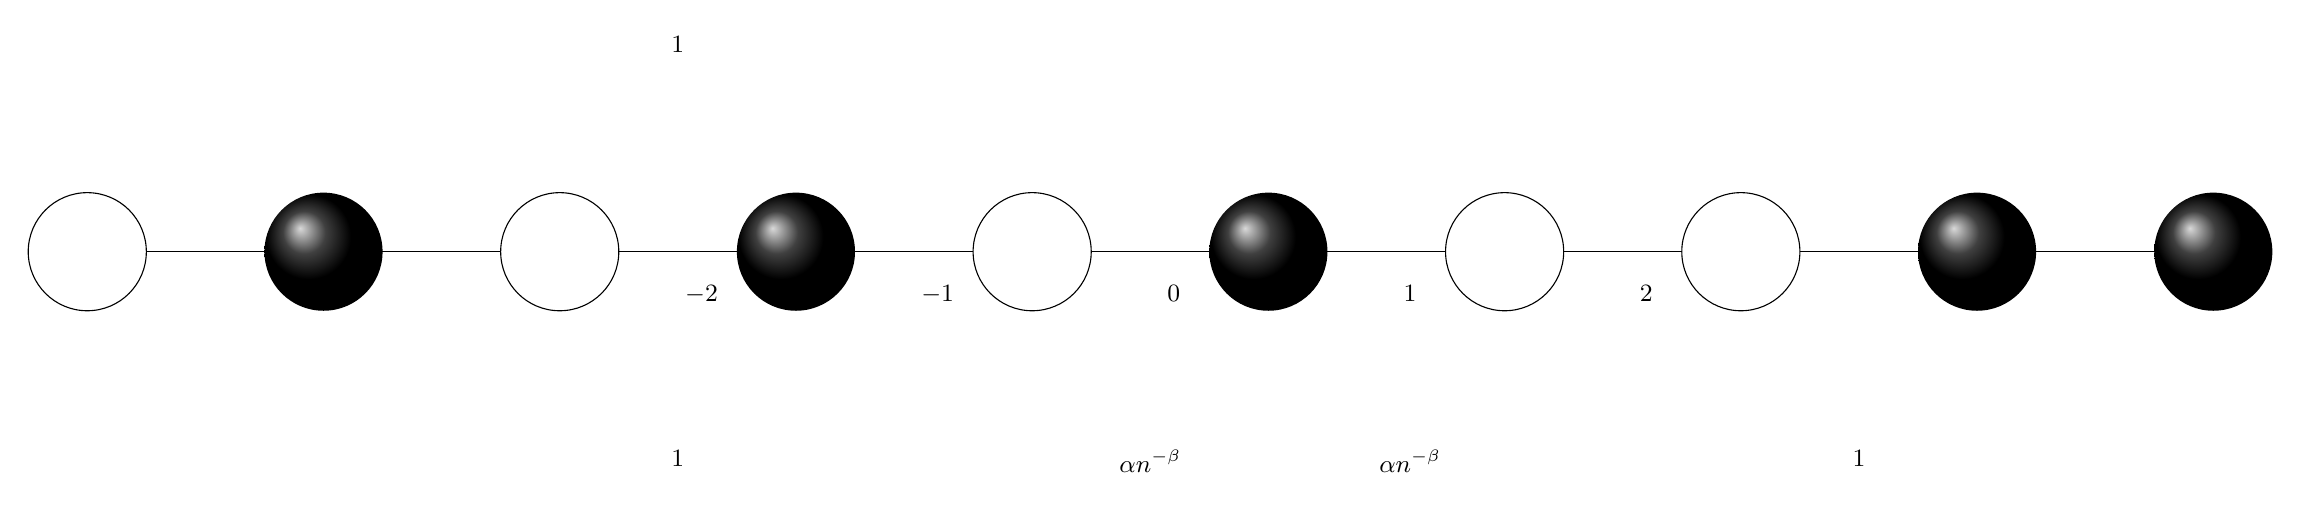
\begin{tikzpicture}[scale=3]
	%%%%%%arcos%%%%%%%%%%%%%
	\centerarc[thick,<-](2.5,0.3)(10:170:0.45);
	\centerarc[thick,->](2.5,-0.3)(-10:-170:0.45);
	\centerarc[thick,->](4.5,-0.3)(-10:-170:0.45);
	\centerarc[thick,<-](5.5,-0.3)(-10:-170:0.45);
	\centerarc[thick,<-](4.5,0.3)(10:170:0.45);
	\centerarc[thick,->](7.5,-0.3)(-10:-170:0.45);
	%\centerarc[thick,<-](7.5,0.3)(10:170:0.45);
	
	%%%%%%%%%%%%%%segmento%%%%%%%%%
	\draw (0,0) -- (9,0);
	
	%%%%%%%%%% partículas em azul %%%%%%%%%%%
	\shade[ball color=black](1,0) circle (0.25);
	\shade[ball color=black](3,0) circle (0.25);
	\shade[ball color=black](5,0) circle (0.25);
	\shade[ball color=black](8,0) circle (0.25);
	\shade[ball color=black](9,0) circle (0.25);
	
	%%%%%%%%%%% partículas em branco %%%%%%%%%%%
	\filldraw[fill=white, draw=black]
	(0,0) circle (.25)
	(2,0) circle (.25)
	(4,0) circle (.25)
	(6,0) circle (.25)
	(7,0) circle (.25);
	
	%%%%%%%%%% rótulos %%%%%%%%%%%%%%
	\draw
	(2.6,-0.1) node[anchor=north] {\small $-2$}
	(3.6,-0.1) node[anchor=north] {\small $-1$}
	(4.6,-0.1) node[anchor=north] {\small $0$}
	(5.6,-0.1) node[anchor=north] {\small $1$}
	(6.6,-0.1) node[anchor=north] {\small $2$};
	\draw (2.5,0.8) node[anchor=south]{\small $1$};
	\draw (2.5,-0.8) node[anchor=north]{\small $1$};
	\draw (5.5,-0.8) node[anchor=north]{\small \hspace{0.6cm}$\alpha n^{-\beta}$};
	\draw (7.5,-0.8) node[anchor=north]{\small $1$};
%	\draw (4.5,0.8) node[anchor=south]{\small $1$};
	\draw (4.5,-0.8) node[anchor=north]{\small $\alpha n^{-\beta}$};
	\end{tikzpicture}
	\caption{At most one particle per site. A particle at the origin jumps at a lower rate $\alpha n^{-\beta}$.}
\end{figure}

In order to see the process on its diffusive time scaling, we will consider the process $\left\{ \eta_t: t \geq 0  \right\}$ with {\color{olive}  \it \large time speeded up by $n^2$}. We recall from \cite[Proposition 2.1]{slow site} that for any $p \in [0,1]$, the Bernoulli product measure $\nu_p$ defined by
\begin{equation}\label{invariant measure}
\nu_p (\eta; \, \eta(x)=1 )\;=:\;m_p(x)\;=\;\begin{cases}
\frac{p/(\alpha n^{-\beta})}{(1-p)+p/(\alpha n^{-\beta})}, & \text{ if } x=0,\\
p, & \text{ if } x \neq 0,
\end{cases}
\end{equation}
is {\color{olive}  \it  \large reversible} for the process $\left\{ \eta_t: t \geq 0  \right\}$.

\subsection{Hydrodynamics}


The process is defined on $\mathbb{T}_n$. Fix a  profile $\rho_0 : \bb T \to {[0,1]}$, representing the initial density of particles. To avoid uninteresting technical complications, we assume that $\rho_0$ is continuous at all $x\in \bb T\backslash \{0\}$ and bounded from below by a positive constant,
\begin{equation}\label{assumption}
\zeta\;:=\;\inf_{x\in\bb T}\rho_0(x)\;>\;0\,.
\end{equation}
The {\it \color{olive} \large empirical measure} is defined as
\begin{equation}\label{}
  \pi^n_t (d u) = \frac{1}{n} \sum_x \eta_t (x) \delta_{x/n} (du).
\end{equation}

\vskip 0.3cm

\begin{tcolorbox}[colback=blue!5!white, title = {\large Theorem 1 (Law of Large Numbers for the Empirical Measure)}]
Let the initial measure $\left\{ \mu_n; n \in \bb N \right\}$ be a sequence of product measures on $\{0,1\}^{\mathbb{T}_n}$ with marginals given by
\begin{equation}
\mu_n \{\eta: \eta(x) = 1\}= \rho_0 (x/n).
\end{equation}
Then, for every $t>0$, $\pi^n_t (d u)$ converges in the weak topology to $\rho (t,u) du$ in probability as $n \rightarrow \infty$, where $\rho (t,u)$ stands for the unique weak solution of
		\begin{itemize}
			\item the heat equation with {\it  \color{olive} periodic boundary conditions} if $\beta \in [0,1)$;
			\item the heat equation with {\it  \color{olive} Robin boundary conditions} if $\beta =1$;
			\item and the heat equation with {\it \color{olive} Neumann boundary conditions} if $\beta > 1$.
		\end{itemize}
\end{tcolorbox}


\subsection{Equilibrium Fluctuations}

The process is defined on $\mathbb{Z}$. The {\it \color{olive} \large fluctuation field}, which is the linear functional  acting on test functions $H$, is defined  as
\begin{equation*}
\mathcal{Y}_t^n(H)\;=\;\frac{1}{\sqrt{n}}\sum_{x \in \bb Z} H\PP{x} \overline{\eta}_t(x)\,,
\end{equation*}
where  $\overline{\eta}_t(x)=\eta_t(x)-m_p(x)$.

\vskip 0.3cm

\begin{tcolorbox}[breakable, title={Domain of the Test Functions in Different Regimes}]
We will set {\large \color{olive} $\mathcal{S}_\beta$}
\begin{itemize}
	\item  for $\beta \in [0,1)$, as the usual Schwartz space;
	\item  for $\beta=1$, as the space of functions $H:\bb R\to\bb R$ such that
	\begin{enumerate}[(1)]
		\item $H$ is continuous and infinitely differentiable, except possibly  at $x=0$.
		\item $H (0)=\frac{1}{2}\big[H(0^+) + H (0^-)\big]$.
		\item  For all integers $k,\ell\geq 0$,
		\begin{equation*}
		\Vert H \Vert_{k,\ell}\;:=\;\sup_{x \neq 0}\Big|(1+|x|^\ell)
		\,\frac{d^k H}{dx^k} (x)\Big|\;<\;\infty\,.
		\end{equation*}
		\item For any integer $k\geq 0$,
		\[
		\frac{d^{2k+1} H}{dx^{2k+1}}(0^{+})\;=\;
		\frac{d^{2k+1} H}{dx^{2k+1}}(0^{-})
		\;=\; \alpha \, \Big( \frac{d^{2k} H}{dx^{2k}}(0^{+})\;-\;
		\frac{d^{2k} H}{dx^{2k}}(0^{-}) \Big)\,.
		\]
	\end{enumerate}
   \item  for $\beta >1$,  as the space of functions $H:\bb R\to\bb R$ that satisfy $(1), (2')$ below, $(3), (4)$ with $\alpha = 0$,\\
    $(2')$ $H$ is continuous from the right at zero.
   \end{itemize}
\end{tcolorbox}

Denote by $\mathcal{S}'_\beta (\bb R)$ the dual space of $\mathcal{S}_\beta (\bb R)$. We will define $\nabla_\beta$ and $\Delta_\beta$
\begin{itemize}
	\item  for $\beta \in [0,1)$, by the usual first and second space derivatives;
	\item  for $\beta \geq 1$, by
	\begin{equation*}
	\nabla_\beta H(u)=\begin{cases}
	\frac{dH}{du}(u), &  \mbox{if}\,\,\,\,u\neq 0\,,\\
	\lim_{u\to 0^+ }\frac{dH}{du}(u), &\mbox{if}\,\,\,\,u=0\,,
	\end{cases}
	\quad \Delta_\beta H(u)=\begin{cases}
	\frac{d^2H}{du^2}(u), &  \mbox{if}\,\,\,\,u\neq 0\,,\\
	\lim_{u\to 0^+ }\frac{d^2H}{du^2}(u), &\mbox{if}\,\,\,\,u=0\,.
	\end{cases}
	\end{equation*}
\end{itemize}

\begin{tcolorbox}[colback= blue!5!white, title = {\large Theorem 2 (Central Limit Theorem for the Density of Particles)}]
 Fix a horizonal time $T>0$.  Consider the Markov process $\{\eta_{t}: t\geq{0}\}$ starting from the invariant state $\nu_p$. Then, the sequence of processes $\{\mathcal{Y}_{t}^n, 0 \leq t \leq T\}_{ n\in{\bb N}}$ converges in distribution, as $n\rightarrow{+\infty}$, with respect to the 	Skorohod topology 	of $\mathcal{D}([0,T], \mathcal{S}'_\beta (\bb R))$ to   $\mathcal{Y}_t$ 	in $\mathcal{C}([0,T],\mathcal{S}'_\beta (\bb R))$, the generalized Ornstein-Uhlenbeck process  which is the formal solution of the SPDE
\begin{equation}\label{OU}
 d\mathcal{Y}_t= \Delta_{\beta} \mathcal{Y}_t dt+\sqrt{2\chi(p)} \nabla_{\beta} d\mc{W}_t\,
\end{equation}
where $\mathcal{W}_t$ is a Brownian motion on the space of tempered distributions and $\chi (p)=p(1-p)$ is the \textit{compressibility} of the system.
\end{tcolorbox}

\begin{tcolorbox}[title={Remark}]
\begin{enumerate}[(i)]
	\item  As we said before, the case $\beta  > 1$ was proved earlier in \cite{slow site}.
	\item  The rigorous meaning of \eqref{OU} is given in terms of martingale problems, see \cite{phaset,slow site} for similar definitions.
\end{enumerate}
\end{tcolorbox}

\section{Strategy of the Proof}


\begin{itemize}
	\item To  prove the hydrodynamic limit when $\beta \in [0,1)$, we use  the {\it \color{olive} \large entropy method} of Guo, Papanicolaou and Varadhan \cite{entropy}, after a smart trick partitioning the space of configurations.
	\item To prove the hydrodynamic limit when $\beta=1$, we appeal to { \it \color{olive} \large Gordin's martingale approximation method}  \cite{gordin}.  The method was introduced by Gordin in $1969$ as an approach to obtain central limit theorems for Markov processes.   It basically consists in approximating an additive functional $\int_0^t F(X_s)\, ds$ of a Markov process to a martingale. The idea is the following: given a Markov process $\left\{ X_t; t \geq 0 \right\}$ with generator $\mathcal{L}$ and a function $f$ in the domain of $\mathcal{L}$, the process
	\begin{equation}
	f(X_t)-f(X_0)-\int_0^t \mf {L} \, f(X_s) ds
	\end{equation}
	is a mean-zero martingale with respect to the law of $\left\{ X_t; t \geq 0 \right\}$ (see \cite[Appendix 1, Lemma 5.1]{claudios}). Therefore, if we solve the Poisson equation
	\begin{equation}\label{poisson}
	\mf {L} \,  f = F
	\end{equation}
	for an \textit{appropriate} $f$, we can express the functional $\int_0^t F(X_s) ds$ as the sum of a martingale and a boundary term. This strategy will be used to prove the {\it \color{olive} replacement lemmas} for the case $\beta=1$.
	\item To prove equilibrium fluctuations for both cases, we maintain the usual { \it \large \color{olive} entropy method}, which now works owing to the fact that since we are starting at the stationary measure, we do not need to pay an entropy price.
\end{itemize}

\begin{comment}

By Dynkin's martingale formula (see \cite[Appendix 1, Lemma 5.1]{claudios}),
\begin{equation}
    M_t^n(H) := \<\pi^n_t,H\> - \<\pi_0^n,H\> - \int_0^t n^2 \mf L_{n} \< \pi_s^n, H \> ds
\end{equation}
is a martingale with respect to the natural filtration, which vanishes in $L^2 (\mathbb{P}_{\mu_n})$ as we prove.We denote
\begin{align*}
\nabla_n^{+}H\PP{x}&\;=\;n \, \Big( H\PP{x+1}-H\PP{x} \Big), \qquad\nabla_n^{-}H\PP{x}\;=\;n \,\Big( H\PP{x}-H\PP{x-1} \Big),\\
\Delta_n H\PP{x}&\;=\;n^2\, \Big(H\PP{x+1}+H\PP{x-1}-2H\PP{x}  \Big)\,.
\end{align*}
Thus, for any value $\beta \geq 0$, straightforward computations tell us that we can rewrite the integral of $n^2 \mf L_{n} \< \pi_s^n, H \>$  in the time interval $[0,t]$ as
\begin{align}
&n^{-1} \int_0^t \sum_{x \notin \left\{-1,0,1 \right\}} \Delta_n H\PP{x} \eta_s(x)ds\label{intui1}\\
&+ \int_0^t \eta_s(1) \nabla_n^+ H\PP{1} ds-\int_0^t \eta_s(-1) \nabla_n^- H\PP{-1} ds \label{intui2}\\
&+n\int_0^t \Big( \alpha n^{-\beta} \eta_s(0)(1-\eta_s(1))-\eta_s(1)(1-\eta_s(0))\Big)\Big(H\PP{1}-H\PP{0}  \Big)ds\label{intui3}\\
&+n\int_0^t \Big( \alpha n^{-\beta} \eta_s(0)(1-\eta_s(-1))-\eta_s(-1)(1-\eta_s(0))\Big)\Big(H\PP{-1}-H\PP{0}  \Big)ds\,.\label{intui4}
\end{align}
When $\beta \in [0,1)$, we prove that the sum of (\ref{intui2}), (\ref{intui3}) and (\ref{intui4}) vanishes as $n \to \infty$ for every $H \in C(\bb T)$, then the expected hydrodynamic equation would be the heat equation with periodic boundary conditions. Similarly, if for $\beta=1$ and for every $H \in C(\bb T)$ we prove that
\begin{align}\label{sufficience2}
\lim_{n \to \infty}\bb E_{\mu_n}& \Big[ \Big| \int_0^t n^2 \mf L_{n} \< \pi_s^n, H \> ds - n^{-1} \int_0^t \sum_{x \notin \left\{-1,0,1 \right\}} \Delta_n H \PP{x} \eta_s(x)ds\\
& -\int_0^t \eta_s(1)\nabla_n^+ H\PP{1}  ds + \int_0^t\eta_s(-1)\nabla_n^- H\PP{-1} ds \nonumber\\
&-{\alpha}\int_0^t (\eta_s(-1)-\eta_s(1)) \Big(H\PP{1}-H\PP{-1}  \Big) ds\Big|\Big] \;=\;0\nonumber\,,
\end{align}
then the hydrodynamic equation must be  the heat equation with Robin boundary conditions.  Last, but not least, for $\beta>1$ and for every $H \in C(\bb T)$ we have
\begin{align}\label{sufficience3}
\lim_{n \to \infty}\bb E_{\mu_n}& \Big[ \Big| \int_0^t n^2 \mf L_{n} \< \pi_s^n, H \> ds - n^{-1} \int_0^t \sum_{x \notin \left\{-1,0,1 \right\}} \Delta_n H \PP{x} \eta_s(x)ds\\
& -\int_0^t \eta_s(1)\nabla_n^+ H\PP{1} ds + \int_0^t\eta_s(-1)\nabla_n^- H\PP{-1}  ds\Big|\, \Big] \;=\;0\nonumber\,,
\end{align}
then the hydrodynamic equation must be  the heat equation with Neumann boundary conditions.
\end{comment}

{\footnotesize

\begin{thebibliography}{10}\label{bibliography}
	
	\bibitem{tavium} Baldasso, R., Menezes, O., Neumann, A., and Souza, R. R.  \textit{Exclusion process with slow boundary.} Journal of Statistical Physics 167.5 (2017): 1112-1142.
	
	\bibitem{navier-stokes} Beltr\'an, J., and C. Landim. \textit{A lattice gas model for the incompressible Navier-Stokes equation.} Annales de l'IHP Probabilités et statistiques. Vol. 44. No. 5. 2008.
	
	\bibitem{demasi} De Masi, A., et al. \textit{Current reservoirs in the simple exclusion process.} Journal of Statistical Physics 144.6 (2011): 1151.
	
	\bibitem{cor} De Masi, A., et al. \textit{Truncated correlations in the stirring process with births and deaths.} Electronic Journal of Probability 17 (2012).
	
	\bibitem{bir-dea} De Masi, A., Presutti, E. and Tsagkarogiannis, D., Vares, M.E., \textit{Non-equilibrium stationary state for the SEP with births and deaths}. Journal of Statistical Physics (2012).
	
	\bibitem{mari2} Erhard, D., Franco, T., Gon\c calves, P., Neumann, A., and Tavares, M. (2018). \textit{Non-equilibrium fluctuations for the SSEP with a slow bond.} arXiv preprint arXiv:1809.04367.
	
	\bibitem{eqflsby} Franco, T., Gon\c calves, P., and Neumann, A. \textit{Equilibrium Fluctuations for the Slow Boundary Exclusion Process.} Meeting on Particle Systems and PDE's. Springer, Cham, 2015.
	
	\bibitem{sbonds} Franco, T., Gon\c calves, P., and Neumann, A. \textit{Hydrodynamical behavior of symmetric exclusion with slow bonds.} Annales de l'IHP Probabilit\'es et statistiques. Vol. 49. No. 2. 2013.
	
	\bibitem{phaset} Franco, T., Gon\c calves, P., and Neumann, A. \textit{Phase transition in equilibrium fluctuations of symmetric slowed exclusion.} Stochastic Processes and their Applications 123.12 (2013): 4156-4185.
	
	\bibitem{unicidade} Franco, T., Gon\c calves, P. and Neumann, A. \textit{Phase transition of a heat equation with Robin’s boundary conditions and exclusion process.} Transactions of the American Mathematical Society 367.9 (2015): 6131-6158.
	
	\bibitem{slow site} Franco, T., Gon\c calves, P. and Sch\"utz, G. M. \textit{Scaling limits for the exclusion process with a slow site.} Stochastic Processes and their applications 126.3 (2016): 800-831.
	
	\bibitem{mari1} Franco, T., and Tavares, M. \textit{Hydrodynamic Limit for the SSEP with a Slow Membrane.} arXiv preprint arXiv:1809.07911 (2018).
	
	\bibitem{flucslowboundary} Gon\c calves, P., Jara, M., Menezes, O., and Neumann, A. (2018). \textit{Non-equilibrium and stationary fluctuations for the SSEP with slow boundary.} arXiv preprint arXiv:1810.05015.
	
	\bibitem{gordin} Gordin, M. I. \textit{The central limit theorem for stationary processes.} Doklady Akademii Nauk. Vol. 188. No. 4. Russian Academy of Sciences, 1969.
	
	\bibitem{entropy} Guo, M. Z., G. C. Papanicolaou, and S. R. S. Varadhan. \textit{Nonlinear diffusion limit for a system with nearest neighbor interactions.} Communications in Mathematical Physics 118.1 (1988): 31-59.
	
	\bibitem{shiryaev} Jacod, J., and Shiryaev, A. \textit{Limit theorems for stochastic processes.} Springer, 2003.
	
	\bibitem{HS} Holley, R. A., \& Stroock, D. W. (1978). Generalized Ornstein-Uhlenbeck processes and infinite particle branching Brownian motions. Publications of the Research Institute for Mathematical Sciences, 14(3), 741-788.
	
	\bibitem{claudios} Kipnis, C., and Landim, C. \textit{Scaling Limits of Interacting Particle Systems.} Vol. 320. Springer Science and Business Media, 1998.
	
	\bibitem{kipnis-varadhan} Kipnis, C., and Varadhan, S. \textit{Central limit theorem for additive functionals of reversible Markov processes and applications to simple exclusions.} Communications in Mathematical Physics 104.1 (1986): 1-19.
	
	\bibitem{liggett} Liggett, T.M. \textit{ Interacting particle systems.} Vol. 276. Springer Science and Business Media, 2012.
	
	\bibitem{mitoma} Mitoma, I. (1983). Tightness of Probabilities On $ C ([ 0, 1];\mathscr {S}') $ and $ D ([0,1] ;\mathscr {S}') $. The Annals of Probability, 11(4), 989-999.
	
	\bibitem{functional analysis} M. Reed, B. Simon, Functional Analysis, Vol. 1, first ed., in: Methods of Modern Mathematical Physics, Academic Press, 1981.
	
\end{thebibliography}
}
\end{multicols}

\vskip 0.5cm



\begin{minipage}{1.0\linewidth}	
	\thanks{\color{blue} $^{1}$Universidade Federal da Bahia, Brazil,\,
		$^2$Instituto Superior T\'ecnico, Portugal,\,
		$^3$Peking University, China\\[2mm]
		{\it Email:}
		tertu@ufba.br, \, patricia.goncalves@math.tecnico.ulisboa.pt, \, rodrigo.marinho@tecnico.ulisboa.pt  \, and \, zhaolinjie@pku.edu.cn}
\end{minipage}

\end{document} 